\section{Design of Model}
First we denote the following notations.
\begin{table}[H]
\centering
\caption{Notation}
\label{not}
\begin{tabular}{l|l}
\hline
$S_0$& current stock price\\
$S_t$& stock price at time t\\
$K$& strike price determined in the options\\
$r$& interest rate\\
$T$& the maturity of the corresponding option\\
$M$& time steps in binomial model\\
$u$& up factor in binomial Model\\
$q$& R.N. probability in binomial model for price going up\\
$c$& theoretical price of the European call/put option\\
$\bar{c}$& the market price of the European call/put option\\
$\sigma$& the volatility of the underlying stock\\
$\sigma_m$& the implied volatility \\
$opType$& option type, call or put\\
\hline
\end{tabular}
\end{table}\noindent
\subsection{Build binomial model}
We used discrete binomial option pricing model for this project.\\
About how to build the model, please refer to memo and python file in Appendix 1.
\subsection{Methods to get $u$}
After building the model, the key problem becomes how can we get this $u$ factor. We used 4 different methods to do this. 
\subsubsection{up/down factor method}
\paragraph{Step1:} First find all ATM option data--($S_0,K,r,T,M,opType,c$) based on current stock price.
\paragraph{Step2:} define function $F(u)=\text{crrModel.payoff}(S_0,K,r,u,T,M,opType)-c$
\paragraph{Step3:} use a non-linear solver to solve $F(u)=0$
For following volatility related methods, we calculate $u$ from volatilities using $u=e^{\sigma\sqrt{T/M}}$.\cite{Bible}
\subsubsection{implied volatilities}
Suppose the Black-Scholes Model for option pricing is:
$c=f(\sigma,.)$, then implied volatility is given by $\sigma_m=f^{-1}(\bar{c},.)$. In practice, we find the root of function: $f(\sigma_m,.)-\bar{c}=0$. We used python package \textit{mibian}for  Black-Scholes Model. Please check Part3 from Appendix 2 for this.
\subsubsection{volatility based on historical data}
This method is to estimate the volatility from historical data. In order to estimate the volatility of the stock price, the stock price at some fixed intervals of time needs to be observed. In this project, $n+1$ is used to denote the number of observations, $S_i$ is used to denote the stock price at the end of $i^{th}$ interval, where i takes values in 0,1,2,…,n., and t is used to denote the length of time interval in years.
\paragraph{Step1: computation for daily volatility}
The goal of this part is to computing the daily volatility by using the formula $u_i=\log(\frac{S_i}{S_{i-1}})$
The data which is used here is from June 26, 2014 to November 5, 2014. The length of this period is the same as the length of the period from today to the expiration day of the option. So the annual volatility can be estimated in the future by using the historical data from June 26 till now.
\paragraph{Step2: estimating the standard deviation of $u_i$}
The estimated $s$ can be computed by using the formula $s=\sqrt{\frac{\sum_{i=1}^{n}(u_i-\bar{u})^2}{n-1}}$
\paragraph{Step3: computation for annual volatility}
The estimated $s$, which is the standard deviation of the daily return, has to be converted into the volatility per annum. Assume there are 252 trading days per year, the volatility per annual is $s*\sqrt{252}$.\cite{Bible}
\subsubsection{volatility using GARCH}
GARCH is the abbreviation of Generalized AutoRegressive Conditional Heteroskedasticity. The distinctive feature of the model is that it acknowledge that volatilities and correlations are not constants. The model attempts to keep track of the variations in the volatility or correlation through time. It is often used to analyse financial data. GARCH (1,1) is the most popular of the GARCH models.\cite{BSG} \\
We use $\sigma_n$ denote the volatility of a market on day $n$, which is estimated at the end of day n-1. The square of the volatility, $\sigma_n^2$, on day $n$ is the variance rate. We assume the value of the market variable at the end of the day $i$ is $S_i$. Also, we use variable $u_i$ denote the continuously compound return during day $i$.
\begin{equation}
u_i=\frac{S_i-S_{i-1}}{S_{i-1}}
\end{equation}
In the GARCH (1,1) model, $\sigma_n^2$ is calculated from a long-run average variance rate, $V_L$, as well as from $\sigma_{n-1}$ and $u_{n-1}$. The equation for the model is 
\begin{equation}
\sigma_n^2=r V_L +\alpha u_{n-1}^2+\beta \sigma_{n-1}^2
\end{equation}
Then an unbiased estimate of the variance rate per day, $\sigma_n$, using the most recent $m$ observations on the market is $\sigma_n^2=\frac{1}{m-1}\sum_{m}^{i=1}(u_i-\bar{u})^2$\\
The term (p, q) of the GARAH (p, q) means that  is based on the most recent p observations of and the most recent q estimate of the variance rate. The (1, 1) term is the most common used one in the GARCH models.\cite{GARCH}\\
Let $\omega=r V_L$, we can rewrite the model as 
\begin{equation}
\sigma_n^2=\omega+\alpha u_{n-1}^2+\beta \sigma_{n-1}^2
\end{equation}
This form is frequently used for estimating the parameters.
\paragraph{Step 1: Choose the sample of our model}
Three months volatility of the stock price is computed by using the historical data. Three months volatility makes sense here because the period from now to the expiration day of the option is about three months and the forecast value will be more accurate. The close price of GE from November 5, 2010 to November 5, 2014 was chosen as the samples.
\paragraph{Step 2: Compute the historical volatility of every three month of the sample space}
The volatility of the stock price of every three months can be computed by the samples. 
\paragraph{Step 3: Estimate the parameter of GARCH(1,1)}
The coefficient of GARCH(1,1) model can be estimated by EVIEWS.
\paragraph{Step 4: Forecast the volatility of next three months}
Forecast the volatility of the stock price of GE in the next three months by using GARCH (1,1) model. Since the outcome of the forecast is the volatility of three months, and the u and d are computed by the annual volatility, so the three months volatility need to convert into annual volatility.
\section{Calibration}
\subsection{Statistics}
We use two statistics for calibrating the model, errMean and errStd.
They are defined in the following way:\\
$errMean =\mathbb{E}[\frac{|price_{pred} -price_{market}|}{price_{market}}] \quad \quad  errStd=\sqrt{\mathrm{var}[\frac{|price_{pred} -price_{market}|}{price_{market}}]}$\\
\\
Note this is the relative error of predicted option price.\\
The first column of the table indicates the method, note there are nine different $u$ to choose for up/down factor methods.  \\
imVola means implied volatility is used(calculated by ourself). imVolaGiven used given implied volatility on yahoo.finance.\\
hisVola is volatility calculated by historical data. garchVola is volatility get from GRACH method.\\
From the results we can pick out the best $u$ for up/down factor method, which is $u=1.007315$ for call option and $u=1.009611$ for put option.
We can also compare these four methods based on this results. Implied volatility seems to perform best among the four, with $5\%$ error for call option and $9\%$ error for put option.\\

\begin{table}[H]
\centering
\caption{error statistics for call options}
\label{errc}
\begin{tabular}{l|l|l}
\hline
\textbf{u}&\textbf{errMean}&\textbf{errStd}\\
\hline
1.0084473613&0.232986975094&0.31327168106\\
1.00961093521&0.352464003312&0.455026566863\\
1.00731514523&0.188305741618&0.313810653125\\
1.00755989205&0.189470517888&0.30527422953\\
1.00683422169&0.201975445117&0.331794778452\\
1.00804336626&0.207643935028&0.299982554264\\
1.00709275526&0.192770213663&0.321432952658\\
1.00819095924&0.214498332689&0.303342310173\\
1.00725089647&0.189207566397&0.31581231149\\
imVola&0.0505378834343&0.0843678348481\\
imVolaGiven&0.0448397508013&0.0723158330639\\
hisVola&0.193911239052&0.301018401547\\
garchVola&0.329698783236&0.390333582641\\
\hline
\end{tabular}
\end{table}\noindent

\begin{table}[H]
\centering
\caption{error statistics for put options}
\label{errp}
\begin{tabular}{l|l|l}
\hline
\textbf{u}&\textbf{errMean}&\textbf{errStd}\\
\hline
1.0084473613&0.60674063871&0.400081408063\\
1.00961093521&0.564245956315&0.404760883793\\
1.00731514523&0.65367226676&0.383312211102\\
1.00755989205&0.644074662439&0.386925369376\\
1.00683422169&0.671691659253&0.37749829154\\
1.00804336626&0.624208642415&0.394064409419\\
1.00709275526&0.662189928282&0.38042940678\\
1.00819095924&0.617735419942&0.396344616465\\
1.00725089647&0.656141017274&0.38243926609\\
imVola&0.0965905974612&0.17889593364\\
imVolaGiven&0.189867073335&0.274381940521\\
hisVola&0.638018294857&0.388996733062\\
garchVola&0.728728309805&0.362709765342\\
\hline
\end{tabular}
\end{table}





\subsection{Plots}
We did the plots for all four methods. Both predicted price and market price are plotted against strike price. We did this for all options listed on yahoo.finance.\\
Figure 1 and 2 are results using up/down factor method.\\
Figure 3 and 4 are results using historical volatility method.\\
Figure 5 and 6 are results using GARCH volatility method.\\
Figure 7 and 8 are results using implied volatility method.
\begin{landscape}
\begin{figure}[H]
\centering
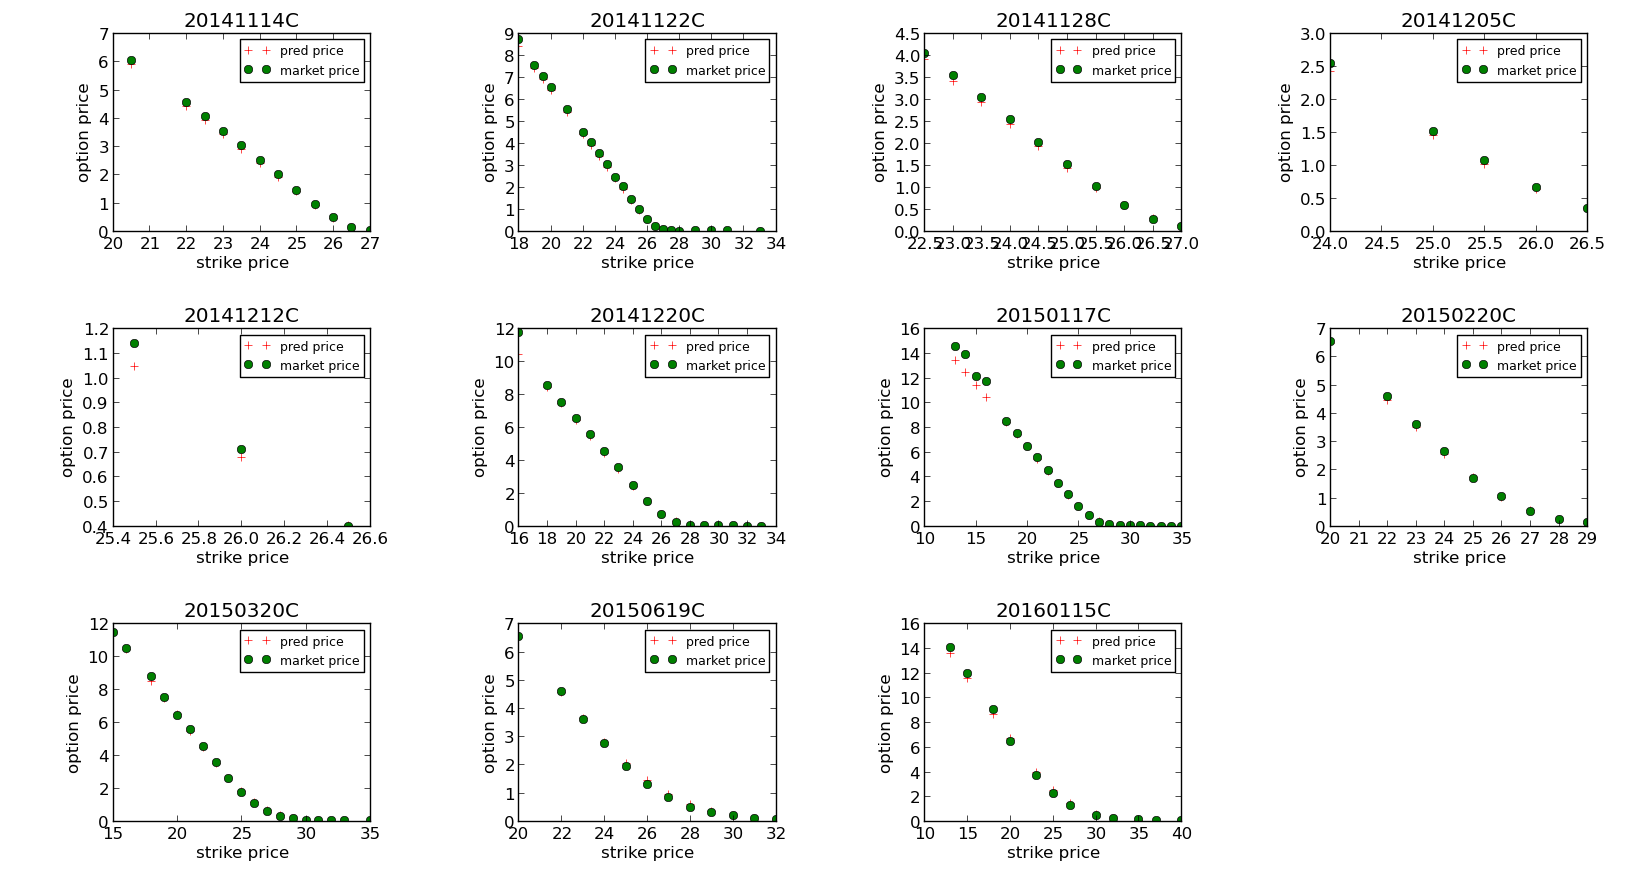
\includegraphics[width=\linewidth]{ucall.png}
\caption{call option price, $u=1.007315$}
\end{figure}
\begin{figure}[H]
\centering
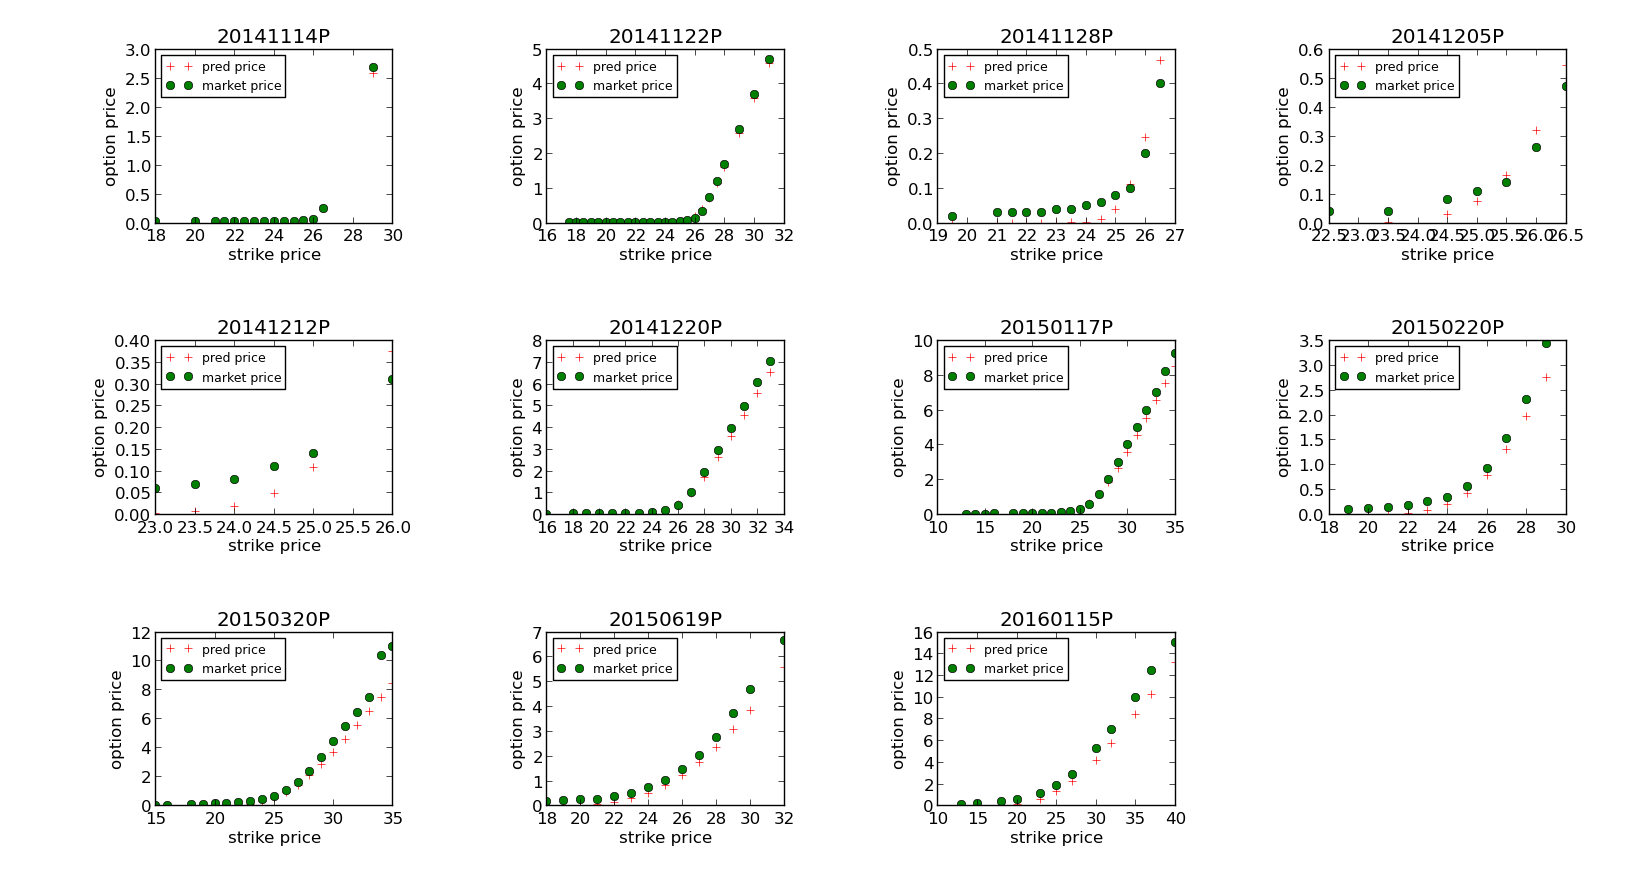
\includegraphics[width=\linewidth]{uput.png}
\caption{put option price, $u=1.009611$}
\end{figure}

\begin{figure}[H]
\centering
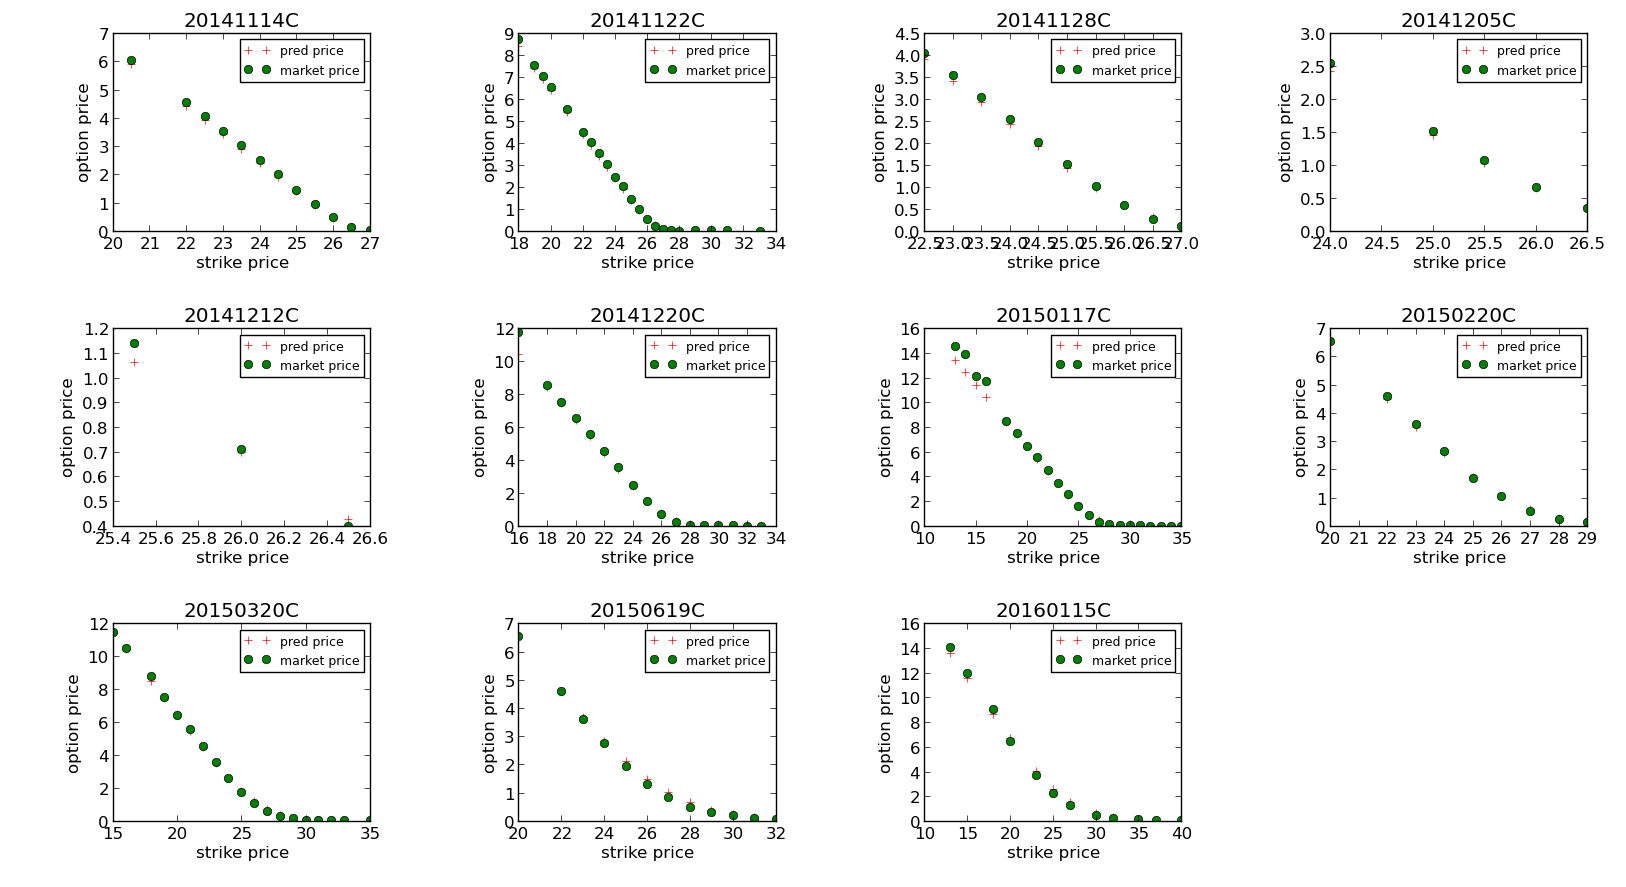
\includegraphics[width=\linewidth]{hisVolaCall.png}
\caption{call option price using historical volatility}
\end{figure}
\begin{figure}[H]
\centering
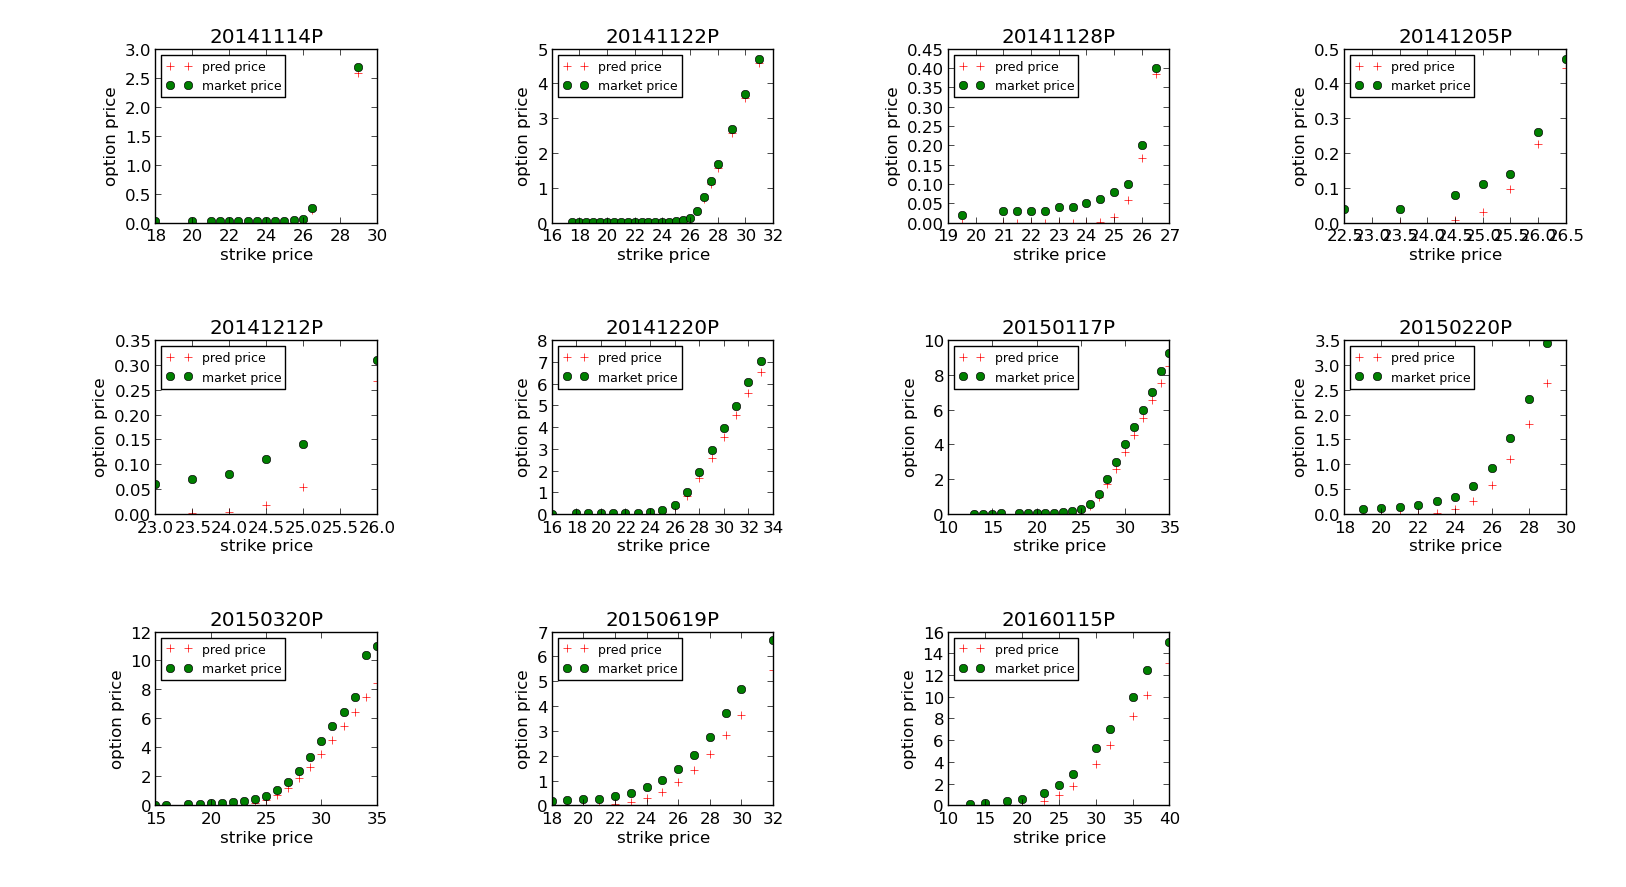
\includegraphics[width=\linewidth]{hisVolaPut.png}
\caption{put option price using historical volatility}
\end{figure}

\begin{figure}[H]
\centering
\includegraphics[width=\linewidth]{GARCHVolaCall.png}
\caption{call option price using GARCH volatility}
\end{figure}
\begin{figure}[H]
\centering
\includegraphics[width=\linewidth]{GARCHVolaPut.png}
\caption{put option price using GARCH volatility}
\end{figure}

\begin{figure}[H]
\centering
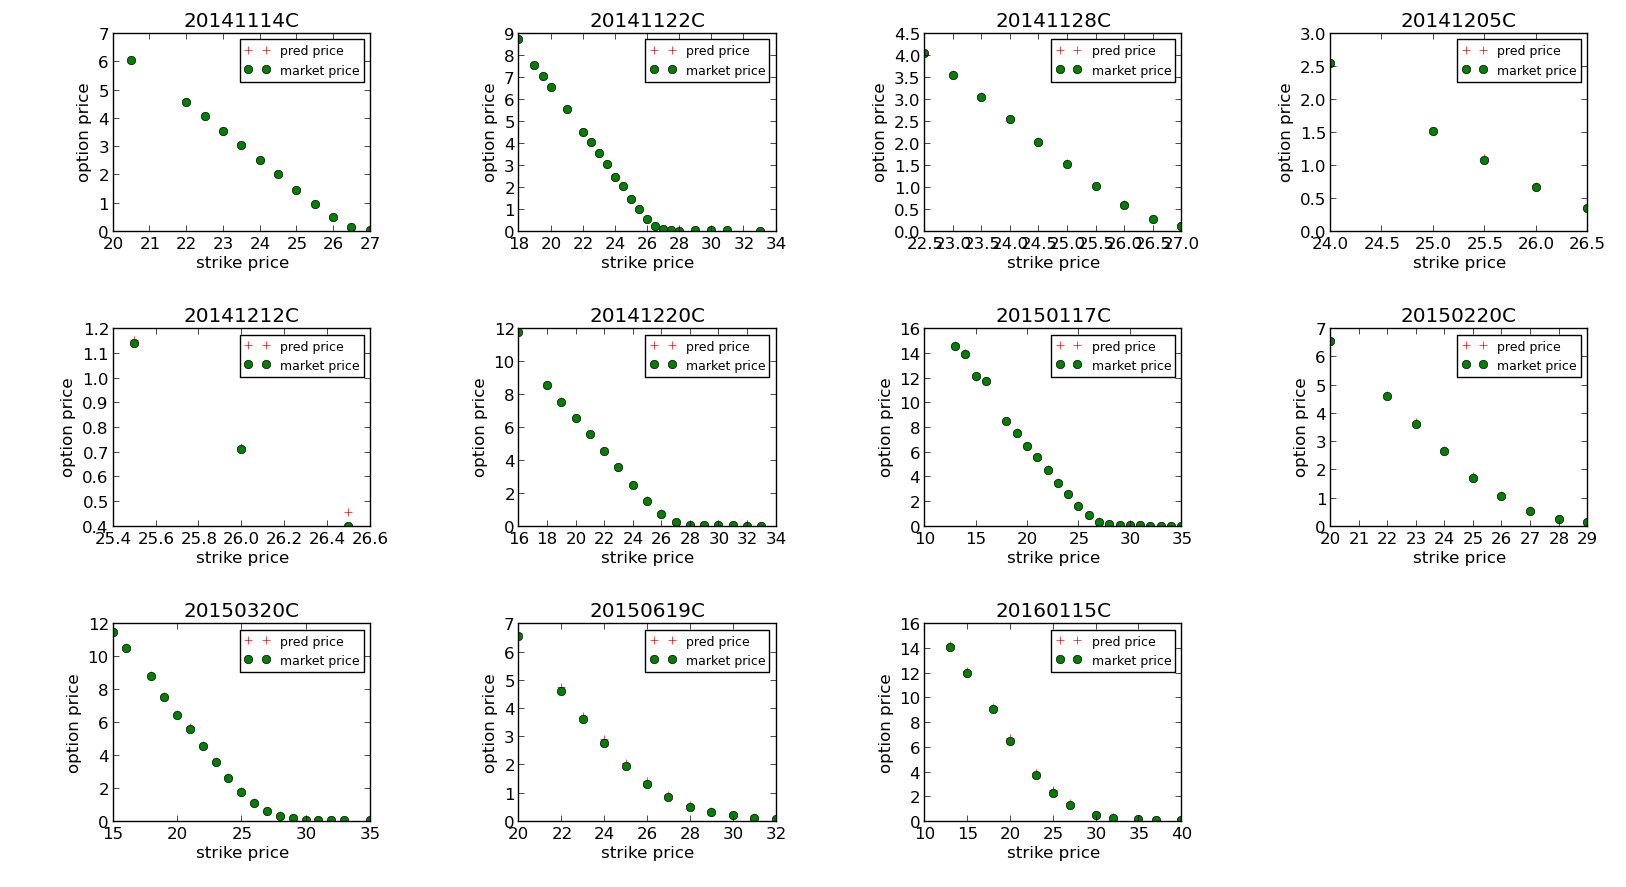
\includegraphics[width=\linewidth]{imVolaCall.png}
\caption{call option price using implied volatility}
\end{figure}
\begin{figure}[H]
\centering
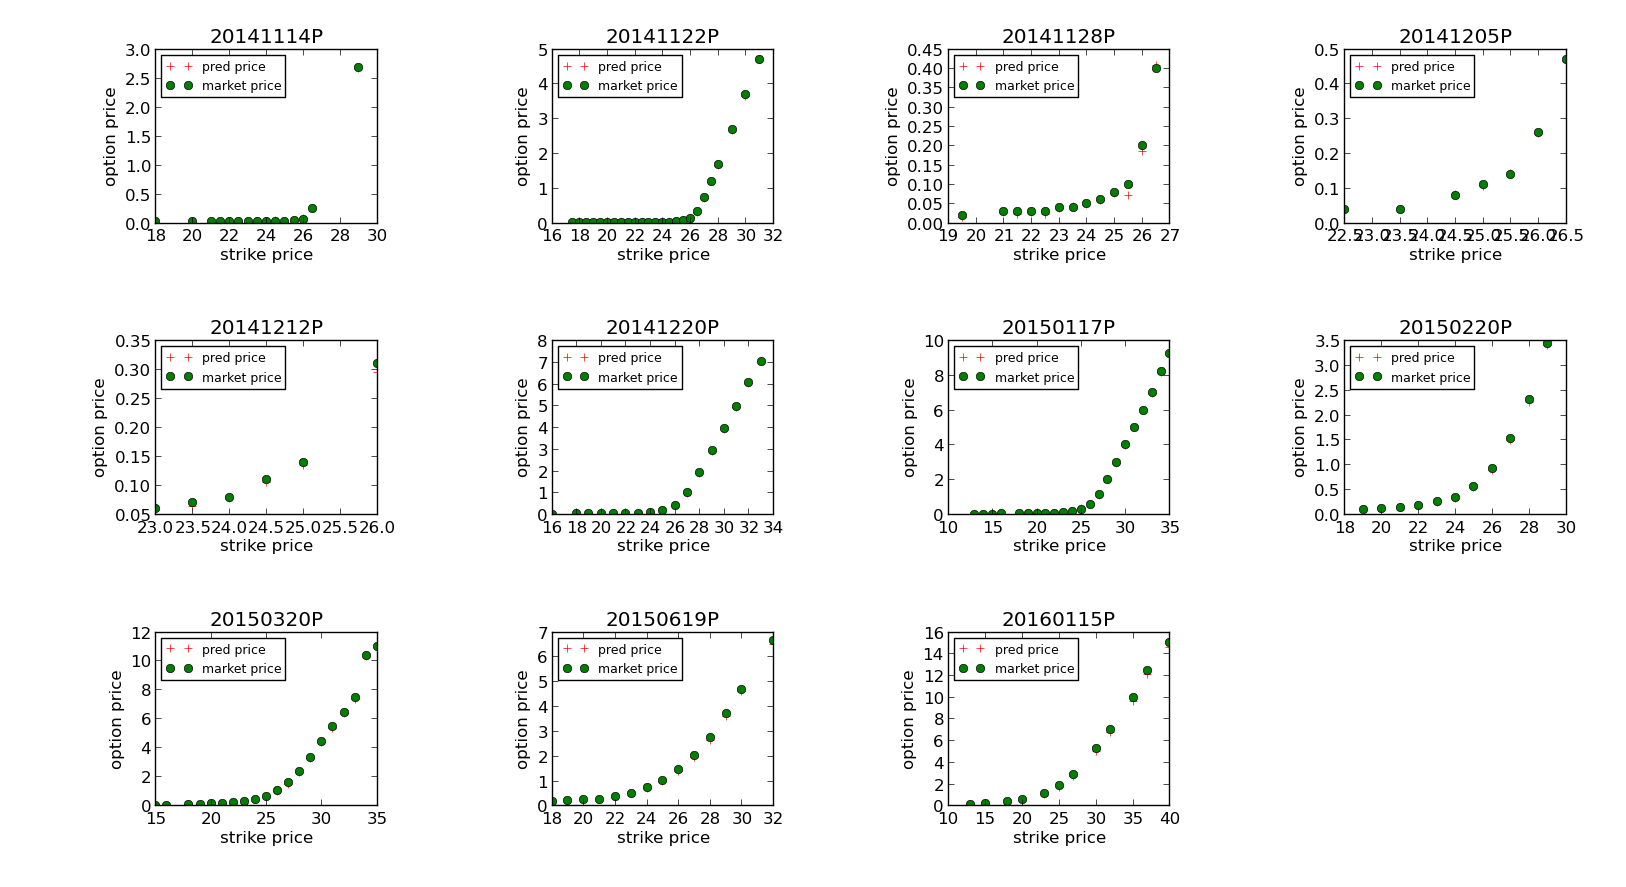
\includegraphics[width=\linewidth]{imVolaPut.png}
\caption{put option price using implied volatility}
\end{figure}
\end{landscape}



\section{Explanation}
From the above results, we can see using a fixed up/down factor method have a big error 20\% for calls,60\% for puts. Fixed volatility method are even worse, historical are better than GARCH and had a similar error as up/down factor method. This makes sense since we know the volatility has a smile curve and shouldn't be fixed values.\\
The best method should be implied volatility method, which is also predictable. Because what we did is using Black-Schole Model to compute implied volatility and plug it back to binomial model, and we know with large $M$, binomial will converge to Black-Schole Model. Hence, we should get a close value since what we did is similar to $F(F^{-1}(c_0))=c_0$\\
However, using given implied volatility we get a bigger error than using calculated ones. This means the models we use are different from the model for market quotes. In fact, we found the given implied volatility are flatter than the calculated ones, so we think the model they used may have jumps(for example Levy process).\\
Finally, there is a big difference of errors for put and call option. We think this may resulted by too many zeros prices for put options.\\
\newpage
\section{Pricing GE option (maturity March 15 2015)}
Based on the previous step, implied volatility method seems to have best performance.
However, since there is no option quotes for maturity at March 15 2015 we can't use implied volatility. Instead we use up/down factor method which is second best among the four.\\
We calculated the price separately, with Table \ref{marc} for call options and Table \ref{marp} for put options.\\
\begin{table}[H]
\centering
\caption{Mar 15,2015 call option pricing using crr model ($u=1.007315$)}
\label{marc}
\begin{tabular}{l|l|l|l}
\hline
\textbf{terDate}&\textbf{opType}&\textbf{strike price}&\textbf{option price}\\
\hline
20150320&call&15.0&11.461282001246699\\
20150320&call&16.0&10.464700801353789\\
20150320&call&18.0&8.47153864941777\\
20150320&call&19.0&7.4749642726694931\\
20150320&call&20.0&6.4784966311719181\\
20150320&call&21.0&5.4829452187317358\\
20150320&call&22.0&4.4924554541957704\\
20150320&call&23.0&3.5213405813841572\\
20150320&call&24.0&2.6023390848848038\\
20150320&call&25.0&1.7868116952216715\\
20150320&call&26.0&1.1244037468974664\\
20150320&call&27.0&0.63865629860344442\\
20150320&call&28.0&0.33042940859411701\\
20150320&call&29.0&0.15175046822042076\\
20150320&call&30.0&0.063501731314656626\\
20150320&call&31.0&0.02402151939562441\\
20150320&call&32.0&0.0081636703833747361\\
20150320&call&33.0&0.002507714114669486\\
20150320&call&35.0&0.00018172046078672249\\
\hline
\end{tabular}
\end{table}\noindent

\begin{table}[H]
\centering
\caption{Mar 15,2015  put option pricing using crr model ($u=1.009611$)}
\label{marp}
\begin{tabular}{l|l|l|l}
\hline
\textbf{terDate}&\textbf{opType}&\textbf{strike price}&\textbf{option price}\\
\hline
20150320&put&15.0&9.7867179963705859e-09\\
20150320&put&16.0&3.6325419023585853e-07\\
20150320&put&18.0&7.639062809058851e-05\\
20150320&put&19.0&0.00057746451374074057\\
20150320&put&20.0&0.0030596500184336423\\
20150320&put&21.0&0.013060676245928219\\
20150320&put&22.0&0.041849964937799349\\
20150320&put&23.0&0.1136019753043295\\
20150320&put&24.0&0.25774564177442444\\
20150320&put&25.0&0.50647277601371621\\
20150320&put&26.0&0.88537267682497467\\
20150320&put&27.0&1.4046909519551112\\
20150320&put&28.0&2.0568312590497917\\
20150320&put&29.0&2.8207176450788012\\
20150320&put&30.0&3.6696609789588552\\
20150320&put&31.0&4.5798043461938622\\
20150320&put&32.0&5.5290513505741883\\
20150320&put&33.0&6.4999793185178305\\
20150320&put&34.0&7.4842697437628178\\
20150320&put&35.0&8.4748829594833452\\
\hline
\end{tabular}
\end{table}\noindent








